\documentclass[autodetect-engine,ja=standard, 11.5pt, a4paper, titlepage]{bxjsarticle}
% fleqn:数式を左詰めにする(titlepageの前に挿入可能)
% titlepage:表紙を独立させる
%\setlength{\mathindent}{50pt}
%-------------------------------------------------------%


\usepackage{graphicx} % Required for inserting images
\usepackage{titlesec}
\usepackage{caption}
\usepackage{amsmath} % 数式用
\usepackage{amssymb}
\usepackage{amsmath}
\usepackage{enumerate} % 箇条書き
\usepackage{comment} % コメントアウト
\usepackage[super]{cite} % 参考文献 上付き
\usepackage[version=4]{mhchem}
\usepackage{booktabs} % tableのmidrule
\usepackage{multirow} % tableのmultirow
\usepackage{float} % [H]で厳密に位置を固定
\usepackage{nccmath} % 数式を左に動かす
\usepackage{mathtools}
\usepackage{empheq}
\usepackage{accents} % \undertildeで下付きチルダ
\usepackage{nccmath} % 数式左寄せ環境fleqn

%-------------------------------------------------------%

\pagestyle{plain} % empty:ページ番号削除

%-------------------------------------------------------%

% セクション・サブセクションの見出しのサイズ
\titleformat*{\section}{\Large} % サイズ・太字
\titleformat*{\subsection}{\large}

%-------------------------------------------------------%

\newcommand{\reference}[0]{\setlength{\hangindent}{18pt}\noindent}
\renewcommand{\refeq}[1]{\eqref{#1}式}
\newcommand{\reffig}[1]{図\ref{#1}}
\newcommand{\reftable}[1]{表\ref{#1}}
\newcommand{\degree}[0]{\mathrm{{}^\circ \hspace*{-0.5pt} C}}
\renewcommand{\deg}[0]{\mathrm{{}^\circ}}
\newcommand{\Vector}[1]{{\mbox{\boldmath$#1$}}}
\newcommand{\tensor}[1]{\undertilde{#1}}

\newcommand{\refcite}[2]{\cite{#1}${}^{\text{#2}}$}
\renewcommand{\citeform}[1]{#1)}
\makeatletter % \usepackage以外で@を含むときはこれで囲む
\renewcommand{\@biblabel}[1]{#1)}
\makeatother

\numberwithin{equation}{section} % 式番号にセクションを併記する場合

\renewcommand{\baselinestretch}{1.3}

%**************************************************************
\begin{document}
%\parindent = 0 pt % 常に字下げなし
\centerline{\LARGE 無機化学}
\centerline{\Large 化学反応式\:総整理}
% \rightline{C1TB5054\;鈴木祐太}
\vskip0.5cm

\vskip.5cm
\section*{中和反応:}
\vspace*{-1cm}
  \begin{figure}[H]\centering
    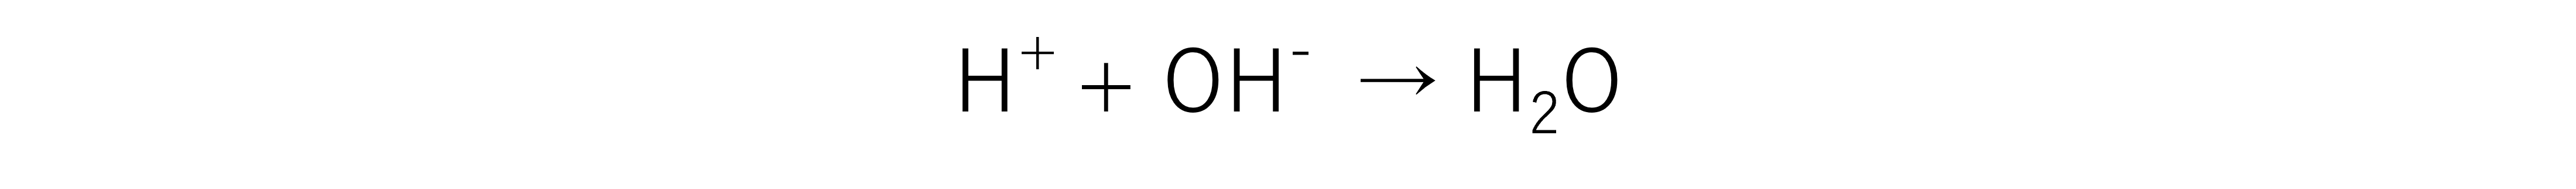
\includegraphics[width=1\linewidth]{asset/1.png}
  \end{figure}
\vspace*{-0.1cm}
\begin{enumerate}[1.]
  \item
  塩酸(硫酸)に水酸化ナトリウム水溶液を加える\\
  \hspace*{10pt}{\large \ce{HCl + NaOH -> NaCl + H2O}}\\
  \hspace*{10pt}{\large (\ce{H2SAO4 + 2 NaOH -> Na2SO4 + 2 H2O})}

  \item
  酢酸水溶液に水酸化ナトリウム水溶液を加える\\
  \hspace*{10pt}{\large \ce{CH3COOH + NaOH -> CH3COONa + H2O}}

  \item
  水酸化アルミニウムに塩酸を加える\\
  \hspace*{10pt}{\large \ce{Al(OH)3 + 3 HCl -> AlCl3 + 3 H2O}}

  \item
  水酸化亜鉛に塩酸を加える\\
  \hspace*{10pt}{\large \ce{Zn(OH)2 + 2 HCl -> ZnCl2 + 2 H2O}}
  \item
  シュウ酸に水酸化ナトリウム水溶液を加える\\
  \hspace*{10pt}{\large \ce{H2C2O4 + 2 NaOH -> Na2C2O4 + 2 H2O}}
  \item
  水酸化カルシウムに塩酸を加える\\
  \hspace*{10pt}{\large \ce{Ca(OH)2 + 2 HCl -> CaCl2 + 2 H2O}}
  \item
  水酸化バリウムに希硫酸を加える\\
  \hspace*{10pt}{\large \ce{Ba(OH)2 + H2SO4 -> BaSO4 + 2 H2O}}
  \item
  アンモニアと塩化水素の反応\\
  \hspace*{10pt}{\large \ce{NH3 + HCl -> NH4Cl}}

\end{enumerate}
\vskip.5cm
\section*{金属元素の酸化物と水の反応:}
\vspace*{-0.5cm}
  \begin{figure}[H]\centering
    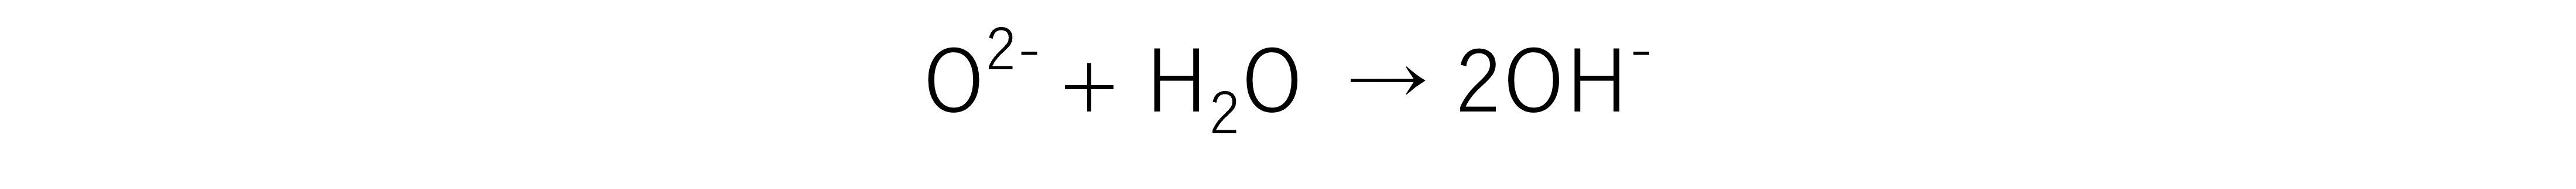
\includegraphics[width=1\linewidth]{asset/2.png}
  \end{figure}
\vspace*{-0.1cm}

\begin{enumerate}[1.]
  \item
  酸化ナトリウムを水に加える\\
  \hspace*{10pt}{\large \ce{Na2O + H2O -> 2 NaOH}}
  \item
  酸化カルシウムを水に加える\\
  \hspace*{10pt}{\large \ce{CaO + H2O -> Ca(OH)2}}
\end{enumerate}
  \hspace*{10pt}補足:\\
  \hspace*{10pt}常温で水と反応する金属元素の酸化物は,アルカリ金属とアルカリ土類金属のみ。

\vskip.5cm
\section*{金属元素の酸化物と酸の反応:}
\vspace*{-0.5cm}
  \begin{figure}[H]\centering
    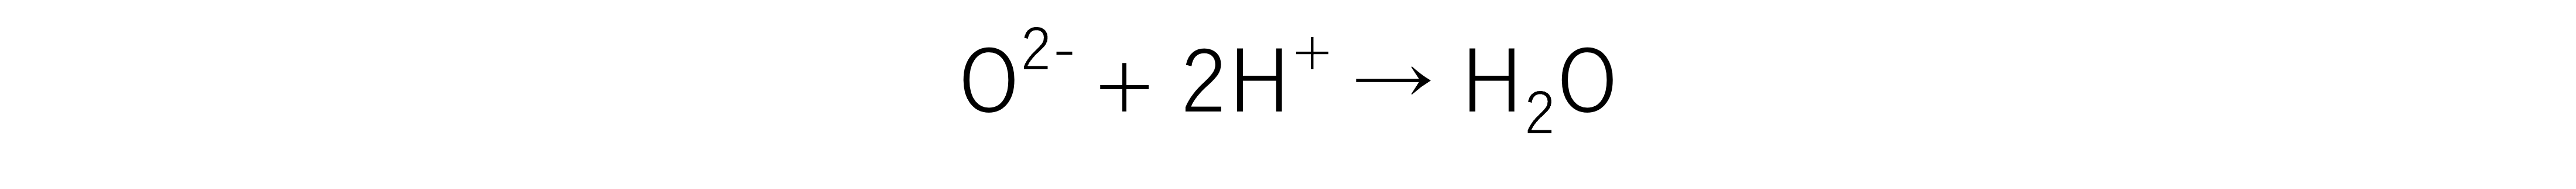
\includegraphics[width=1\linewidth]{asset/3.png}
  \end{figure}
\vspace*{-0.1cm}

\begin{enumerate}[1.]
  \item
  酸化アルミニウムに塩酸(希硫酸)を加える\\
  \hspace*{10pt}{\large \ce{Al2O3 + 6 HCl -> 2 AlCl3 + 3 H2O}}\\
  \hspace*{10pt}{\large (\ce{Al2O3 + 3 H2SO4 -> Al2(SO4)3 + 3 H2O})}
  \item
  酸化亜鉛に塩酸(希硫酸)を加える\\
  \hspace*{10pt}{\large \ce{ZnO + 2 HCl -> ZnCl2 + H2O}}\\
  \hspace*{10pt}{\large (\ce{ZnO + H2SO4 -> ZnSO4 + H2O})}

  \item
  酸化銅(Ⅱ)に希硫酸(希塩酸)を加える\\
  \hspace*{10pt}{\large \ce{CuO + H2SO4 -> CuSO4 + H2O}}\\
  \hspace*{10pt}{\large (\ce{CuO + 2 HCl -> CuCl2 + H2O})}

  \item
  酸化鉄(Ⅲ)に希塩酸を加える\\
  \hspace*{10pt}{\large \ce{Fe2O3 + 6 HCl -> 2 FeCl3 + 3 H2O}}
  \item
  酸化カルシウムに塩酸を加える\\
  \hspace*{10pt}{\large \ce{CaO + 2 HCl -> CaCl2 + H2O}}
\end{enumerate}
\vskip.5cm

\section*{非金属元素の酸化物と水の反応:}
\vspace*{0cm}
  \begin{figure}[H]\centering
    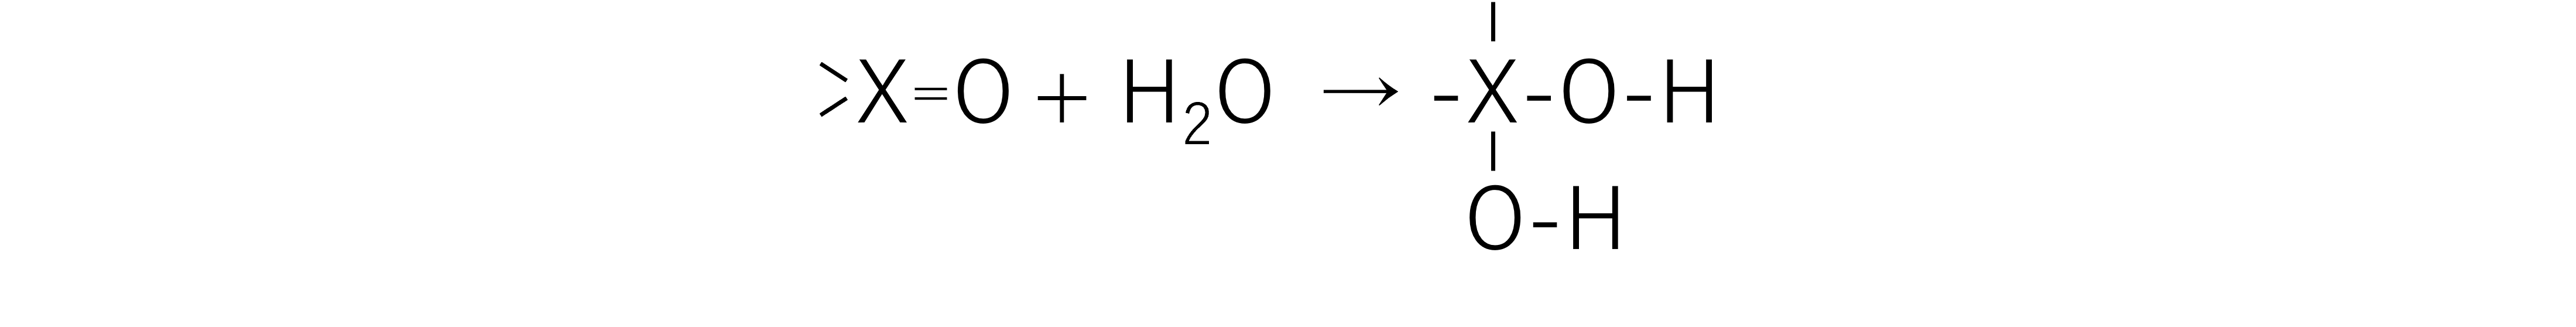
\includegraphics[width=1\linewidth]{asset/4.png}
  \end{figure}
\vspace*{-0.1cm}

\begin{enumerate}[1.]
  \item
  二酸化炭素を水に溶かす\\
  \hspace*{10pt}{\large \ce{CO2 + H2O -> H2CO3}}
  \item
  二酸化硫黄を水に溶かす\\
  \hspace*{10pt}{\large \ce{SO2 + H2O -> H2SO3}}
  \item
  三酸化硫黄を水に溶かす\\
  \hspace*{10pt}{\large \ce{SO3 + H2O -> H2SO4}}
  \item
  十酸化四リンに水を加えて加熱する\\
  \hspace*{10pt}{\large \ce{P4O10 + 6 H2O ->[$\Delta$] 4 H3PO4}}
  \item
  二酸化窒素を温水に溶かす\\
  \hspace*{10pt}{\large \ce{3NO2 + H2O -> 2 HNO3 + NO}}
  \item
  二酸化窒素を冷水に溶かす\\
  \hspace*{10pt}{\large \ce{2NO2 + H2O -> HNO3 + HNO2}}
\end{enumerate}

\vskip.5cm
\section*{非金属元素の酸化物と塩基の反応:}
\vspace*{0cm}
  \begin{figure}[H]\centering
    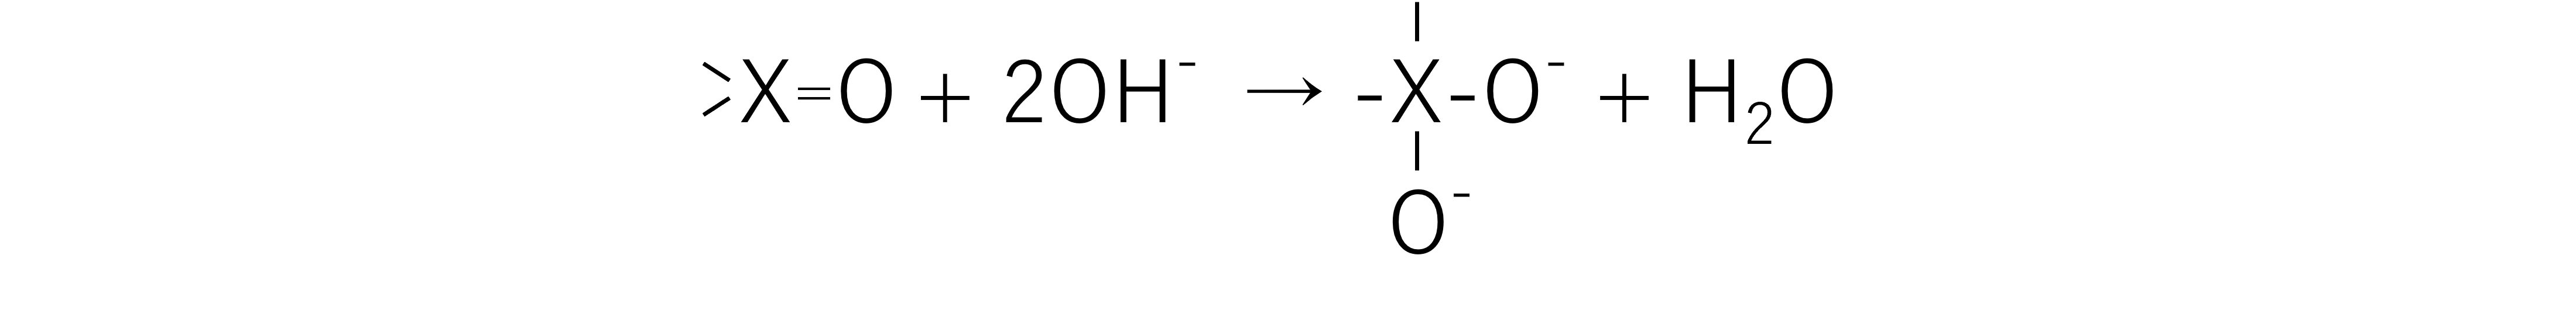
\includegraphics[width=1\linewidth]{asset/5.png}
  \end{figure}
\vspace*{-0.1cm}

\begin{enumerate}[1.]
  \item
  水酸化カルシウム水溶液(石灰水)に二酸化炭素を通じると白濁する\\
  \hspace*{10pt}{\large \ce{Ca(OH)2 + CO2 -> CaCO3 + H2O}}
  \item
  水酸化ナトリウム水溶液に二酸化炭素を通じる\\
  \hspace*{10pt}{\large \ce{2NaOH + CO2 -> Na2CO3 + H2O}}
  \item
  水酸化カリウム水溶液に二酸化硫黄を通じる\\
  \hspace*{10pt}{\large \ce{2KOH + SO2 -> K2SO3 + H2O}}
  \item
  水酸化バリウム水溶液に二酸化炭素を通じると白濁する\\
  \hspace*{10pt}{\large \ce{Ba(OH)2 + CO2 -> BaCO3 + H2O}}
  \item
  二酸化ケイ素を水酸化ナトリウムとともに加熱する\\
  \hspace*{10pt}{\large \ce{2NaOH + SiO2 -> Na2SiO3 + H2O}}
\end{enumerate}

\vskip.5cm
\section*{金属元素の酸化物と非金属元素の酸化物の反応:}


\begin{enumerate}[1.]
  \item
  酸化カルシウムと二酸化ケイ素を混ぜて加熱する\\
  \hspace*{10pt}{\large \ce{CaO + SiO2 ->[$\Delta$] CaSiO3}}
  \item
  酸化カリウムと三酸化硫黄との反応\\
  \hspace*{10pt}{\large \ce{K2O + SO3 -> K2SO4}}
  \item
  酸化カルシウムと二酸化炭素との反応\\
  \hspace*{10pt}{\large \ce{CaO + CO2 -> CaCO3}}
\end{enumerate}

\vskip.5cm
\section*{弱酸(弱塩基)遊離反応:}
\vspace*{-0.5cm}
  \begin{figure}[H]\centering
    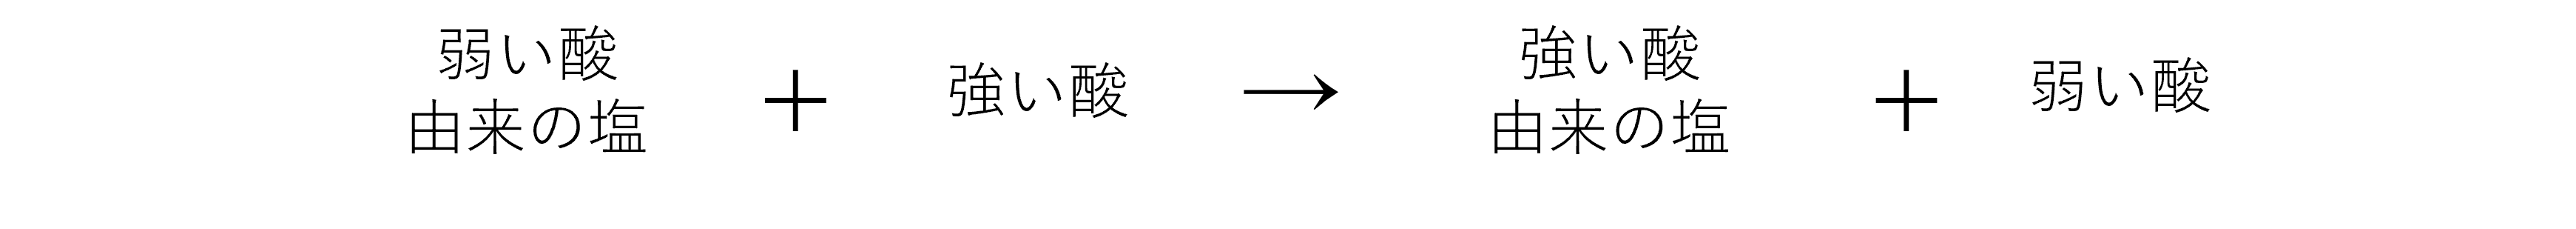
\includegraphics[width=1\linewidth]{asset/6.png}
  \end{figure}
\vspace*{-0.1cm}

\begin{enumerate}[1.]
  \item
  石灰石(炭酸カルシウム)に塩酸を加える\\
  \hspace*{10pt}{\large \ce{CaCO3 + 2 HCl -> CaCl2 + H2O + CO2}}
  \item
  硫化鉄(Ⅱ)に希硫酸(希塩酸)を加える\\
  \hspace*{10pt}{\large \ce{FeS + H2SO4 -> FeSO4 + H2S}}\\
  \hspace*{10pt}{\large (\ce{FeS + 2 HCl -> FeCl2 + H2S})}
  \item
  亜硫酸ナトリウムに希硫酸を加える\\
  \hspace*{10pt}{\large \ce{Na2SO3 + H2SO4 -> Na2SO4 + H2O + SO2}}
  \item
  炭酸ナトリウムに希塩酸を十分に加える\\
  \hspace*{10pt}{\large \ce{Na2CO3 + 2 HCl -> 2 NaCl + H2O + CO2}}
  \item
  ケイ酸ナトリウムに塩酸を加える\\
  \hspace*{10pt}{\large \ce{Na2SiO3 + 2 HCl -> 2 NaCl + H2SiO3}}
  \item
  炭酸カルシウムの沈殿を含む水溶液に二酸化炭素を通じ続ける\\
  \hspace*{10pt}{\large \ce{CaCO3 + H2O + CO2 -> Ca(HCO3)2}}
  \item
  リン酸カルシウムと硫酸を反応させて過リン酸石灰をつくる\\
  \hspace*{10pt}{\large \ce{Ca(PO4)2 + 2 H2SO4 -> 2 CaSO4 + Ca(H2PO4)2}}\\
  \hspace*{10pt}参考:アンモニアと二酸化炭素を高温・高圧下で反応させて尿素をつくる\\
  \hspace*{10pt}{\large \ce{2 NH3 + CO2 -> (NH2)2CO + H2O}}
  \item
  塩化アンモニウムと水酸化カルシウムを混合して加熱する\\
  \hspace*{10pt}{\large \ce{2NH4Cl + Ca(OH)2 ->[$\Delta$] CaCl2 + 2 NH3 + 2 H2O}}
  \item
  塩化鉄(Ⅲ)水溶液を沸騰水に加える\\
  \hspace*{10pt}{\large \ce{FeCl3 + 3 H2O ->[$\Delta$] Fe(OH)3 + 3 HCl}}
\end{enumerate}

\vskip.5cm
\section*{代表的な酸化剤と還元剤の反応:}
\vspace*{-0.5cm}
  \begin{figure}[H]\centering
    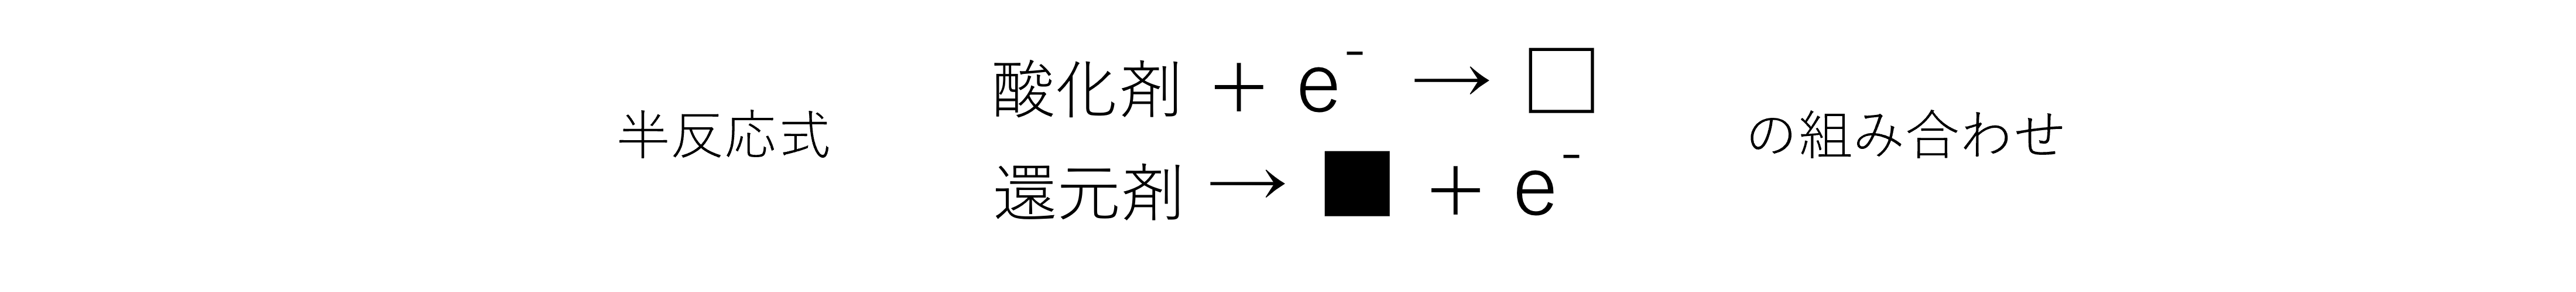
\includegraphics[width=1\linewidth]{asset/7.png}
  \end{figure}


  \begin{table}[H]\caption*{代表的な酸化剤}\label{table:sankazai}
    \centering
    \begin{tabular}{ccccc}
    \toprule
      &名称 & 反応前 &      & 反応後 \\
    \midrule
      1  &\begin{tabular}{c}過マンガン酸イオン\\(酸性溶液中)\end{tabular} & \ce{MnO4-} & \ce{->} & \ce{Mn^{2+}}\\
      2  &二クロム酸イオン & \ce{Cr2O7^{2-}} & \ce{->} & \ce{2 Cr^{3+}} \\
      3  &過酸化水素 & \ce{H2O2} & \ce{->} & \ce{2 H2O} \\
      4  &二酸化硫黄 & \ce{SO2} & \ce{->} & \ce{S} \\
      5  &濃硝酸 & \ce{HNO3} & \ce{->} & \ce{NO2} \\
      6  &希硝酸 & \ce{HNO3} & \ce{->} & \ce{NO} \\
      7  &熱濃硫酸 & \ce{H2SO4} & \ce{->} & \ce{SO2} \\
      8  &塩素 & \ce{Cl2} & \ce{->} & \ce{2 Cl-} \\
      9  &酸素 & \ce{O2} & \ce{->} & \ce{2 H2O} \\
      10 &オゾン & \ce{O3} & \ce{->} & \ce{O2 + H2O} \\
    \bottomrule
    \end{tabular}\end{table}

    \begin{table}[H]\caption*{代表的な還元剤}\label{table:kangen}
    \centering
    \begin{tabular}{ccccc}
    \toprule
      & 名称 & 反応前 &  & 反応後 \\
    \midrule
      11 & ナトリウム & \ce{Na} & \ce{->} & \ce{Na+} \\
      12 & 硫化水素 & \ce{H2S} & \ce{->} & \ce{S} \\
      13 & 二酸化硫黄 & \ce{SO2} & \ce{->} & \ce{SO4^{2-}} \\
      14 & 過酸化水素 & \ce{H2O2} & \ce{->} & \ce{O2} \\
      15 & シュウ酸 & \ce{H2C2O4} & \ce{->} & \ce{2 CO2} \\
      16 & 鉄(Ⅱ)イオン & \ce{Fe^{2+}} & \ce{->} & \ce{Fe^{3+}} \\
      17 & ヨウ化物イオン & \ce{2 I-} & \ce{->} & \ce{I2} \\
      18 & チオ硫酸イオン & \ce{2 S2O3^{2-}} & \ce{->} & \ce{S4O6^{2-}} \\
    \bottomrule
    \end{tabular}\end{table}

    \begin{enumerate}[1.]
      \setlength{\leftskip}{125pt}
      \item \ce{MnO4- + 8 H+ + 5 e- -> Mn^{2+} + 4 H2O}
      \item \ce{Cr2O7^{2-} + 14 H+ + 6 e- -> 2Cr^{3+} + 7 H2O}
      \item \ce{H2O2 + 2 H+ + 2 e- -> 2 H2O}
      \item \ce{SO2 + 4 H+ + 4 e- -> S + 2 H2O}
      \item \ce{HNO3 + H+ + e- -> NO2 + H2O}
      \item \ce{HNO3 + 3 H+ + 3 e- -> NO + 2 H2O}
      \item \ce{H2SO4 + 2 H+ + 2 e- -> SO2 + 2 H2O}
      \item \ce{Cl2 + 2 e- -> 2 Cl-}
      \item \ce{O2 + 4 H+ + 4 e- -> 2 H2O}
      \item \ce{O3 + 2 H+ + 2 e- -> O2 + H2O}
      \item \ce{Na -> Na+ + e-}
      \item \ce{H2S -> S + 2 H+ + 2 e-}
      \item \ce{SO2 + 2 H2O -> SO4^{2-} + 4 H+ + 2 e-}
      \item \ce{H2O2 -> O2 + 2 H+ + 2 e-}
      \item \ce{H2C2O4 -> 2 CO2 + 2 H+ + 2 e-}
      \item \ce{Fe^{2+} -> Fe^{3+} + e-}
      \item \ce{2 I- -> I2 + 2 e-}
      \item \ce{2 S2O3^{2-} -> S4O6^{2-} + 2 e-}
    \end{enumerate}

\begin{enumerate}[1.]
  \item
  硫酸鉄(Ⅱ)と硫酸酸性の過マンガン酸カリウム水溶液を混ぜ合わせる\\
  \hspace*{10pt}{\large \ce{2KMnO4 + 10FeSO4 + 8 H2SO4 -> 2 MnSO4 + K2SO4 + 5 Fe2(SO4)3 + 8 H2O}}
  \item
  ヨウ化カリウム水溶液にオゾンを通じる\\
  \hspace*{10pt}{\large \ce{O3 + 2 KI + H2O -> I2 + O2 + 2 KOH}}
  \item
  過酸化水素水と硫酸酸性の過マンガン酸カリウム水溶液を混ぜ合わせる\\
  \hspace*{10pt}{\large \ce{2KMnO4 + 3 H2SO4 + 5 H2O2 -> 2 MnSO4 + K2SO4 + 5 O2 + 8 H2O}}
  \item
  シュウ酸と硫酸酸性の過マンガン酸カリウムを混ぜ合わせる\\
  \hspace*{10pt}{\large \ce{5(COOH)2 + 2 KMnO4 + 3 H2SO4 -> 2 MnSO4 + 2 K2SO4 + 10CO2 + 8 H2O}}
  \item
  硫酸酸性の過マンガン酸カリウム水溶液に二酸化硫黄を通じる\\
  \hspace*{10pt}{\large \ce{2KMnO4 + 5 SO2 + 2 H2O -> 2 MnSO4 + 2 H2SO4 + K2SO4}}
  \item
  硫酸酸性で過酸化水素水にヨウ化カリウム水溶液を加える\\
  \hspace*{10pt}{\large \ce{H2O2 + H2SO4 + 2 KI -> K2SO4 + I2 + 2 H2O}}
  \item
  ヨウ素溶液に二酸化硫黄を通じる\\
  \hspace*{10pt}{\large \ce{I2 + SO2 + 2 H2O -> H2SO4 + 2 HI}}
  \item
  ヨウ素溶液に硫化水素を通じる\\
  \hspace*{10pt}{\large \ce{I2 + H2S -> S + 2 HI}}
  \item
  水素化ナトリウムを水に加える\\
  \hspace*{10pt}{\large \ce{NaH + H2O -> NaOH + H2}}
  \item
  アルカリ金属(\ce{M})を水に加える\\
  \hspace*{10pt}{\large \ce{2M + 2 H2O -> 2 MOH + H2}}
  \item
  カルシウムを水に加える\\
  \hspace*{10pt}{\large \ce{Ca + 2 H2O -> Ca(OH)2 + H2}}
  \item
  マグネシウムを熱水に加える\\
  \hspace*{10pt}{\large \ce{Mg + 2 H2O ->[$\Delta$] Mg(OH)2 + H2}}
  \item
  アルミニウムを高温の水蒸気に触れさせる\\
  \hspace*{10pt}{\large \ce{2Al + 3 H2O ->[$\Delta$] Al2O3 + 3 H2}}
  \item
  鉄を高温の水蒸気と反応させる\\
  \hspace*{10pt}{\large \ce{3Fe + 4 H2O ->[$\Delta$] Fe3O4 + 4 H2}}
  \item
  亜鉛に希硫酸(希塩酸)を加える\\
  \hspace*{10pt}{\large \ce{Zn + H2SO4 -> ZnSO4 + H2}}\\
  \hspace*{10pt}{\large (\ce{Zn + 2 HCl -> ZnCl2 + H2})}
  \item
  アルミニウムに希塩酸(希硫酸)を加える\\
  \hspace*{10pt}{\large \ce{2Al + 6 HCl -> 2 AlCl3 + 3 H2}}\\
  \hspace*{10pt}{\large (\ce{2Al + 3 H2SO4 -> Al2(SO4)3 + 3 H2})}
  \item
  鉄に希塩酸(希硫酸)を加える\\
  \hspace*{10pt}{\large \ce{Fe + 2 HCl -> FeCl2 + H2}}\\
  \hspace*{10pt}{\large (\ce{Fe + H2SO4 -> FeSO4 + H2})}
  \item
  ハロゲン(X)の単体と水素の反応\\
  \hspace*{10pt}{\large \ce{X2 + H2 -> 2 HX}}\\
  \hspace*{10pt}補足:\\
  \hspace*{10pt}\ce{F2}:爆発的に反応する\\
  \hspace*{10pt}\ce{Cl2}:光照射で爆発的に反応する\\
  \hspace*{10pt}\ce{Br2, I2}:平衡状態になる(\ce{X2 + H2 <=> 2HX})
  \item
  フッ素を水に通じる\\
  \hspace*{10pt}{\large \ce{2F2 + 2 H2O -> 4 HF + O2}}
  \item
  ナトリウムと塩素の反応\\
  \hspace*{10pt}{\large \ce{2Na + Cl2 -> 2 NaCl}}
  \item
  窒素と水素を混合して,高温・高圧で反応させる\\
  \hspace*{10pt}{\large \ce{N2 + 3 H2 <=>[][\ce{Fe}\text{系}] 2 NH3}}

  \item
  ヨウ化カリウム水溶液に塩素を通じる\\
  \hspace*{10pt}{\large \ce{2KI + Cl2 -> I2 + 2 KCl}}
  \item
  ヨウ化カリウム水溶液に臭素を加える\\
  \hspace*{10pt}{\large \ce{2 KI + Br2 -> I2 + 2 KBr}}\\

  \item
  臭化カリウム水溶液に塩素を通じる\\
  \hspace*{10pt}{\large \ce{2 KBr + Cl2 -> Br + 2 KCl}}

  \item
  二酸化硫黄と過酸化水素の反応\\
  \hspace*{10pt}{\large \ce{SO2 + H2O2 -> H2SO4}}

  \item
  二酸化硫黄と硫化水素との反応\\
  \hspace*{10pt}{\large \ce{SO2 + 2 H2S -> 3 S + 2 H2O}}
  \item
  銅に希硝酸を加える\\
  \hspace*{10pt}{\large \ce{3 Cu + 8 HNO3 -> 3 Cu(NO3)2 + 4 H2O + 2 NO}}
  \item
  銅に濃硝酸を加える\\
  \hspace*{10pt}{\large \ce{Cu + 4 HNO3 -> Cu(NO3)2 + 2 H2O + + 2 NO2}}
  \item
  銅に濃硫酸を加えて加熱する\\
  \hspace*{10pt}{\large \ce{Cu + 2H2SO4 ->[$\Delta$] CuSO4 + 2 H2O + SO2}}
  \item
  銀に希硝酸を加える\\
  \hspace*{10pt}{\large \ce{3Ag + 4 HNO3 -> 3 AgNO3  + 2 H2O + NO}}
  \item
  銀に濃硝酸を加える\\
  \hspace*{10pt}{\large \ce{Ag + 2 HNO3 -> AgNO3 + H2O + NO2}}
  \item
  銀に濃硫酸を加えて加熱する\\
  \hspace*{10pt}{\large \ce{2 Ag + 2 HNO3  ->[$\Delta$] Ag2SO4 + 2 H2O + SO2}}
  \item
  酸化マンガン(IV)に濃塩酸を加えて加熱する\\
  \hspace*{10pt}{\large \ce{MnO2 + 4 HCl ->[$\Delta$] MnCl2 + Cl2 + 2 H2O}}
  \item
  さらし粉に塩酸を加える\\
  \hspace*{10pt}{\large \ce{CaCl(ClO)\cdot H2O + 2 HCl -> CaCl2 + Cl2 + 2 H2O}}
  \item
  酸化鉄(Ⅲ)の粉末とアルミニウムの粉末を混合して点火する\\
  \hspace*{10pt}{\large \ce{Fe2O3 + 2 Al ->[$\Delta$] 2 Fe + Al2O3}}
  \item
  酸化鉄(Ⅲ)を一酸化炭素と加熱して還元する\\
  \hspace*{10pt}{\large \ce{Fe2O3 + 3 CO ->[$\Delta$] 2 Fe + 3 CO2}}
  \item
  酸化銅(Ⅱ)を水素と加熱して還元する\\
  \hspace*{10pt}{\large \ce{CuO + H2 ->[$\Delta$] Cu + H2O}}
  \item
  硫化銅(Ⅰ)と酸素を混合して加熱する\\
  \hspace*{10pt}{\large \ce{Cu2S + O2 ->[$\Delta$] 2 Cu + SO2}}
  \item
  リン酸カルシウムと二酸化ケイ素とコークスを混合して加熱する\\
  \hspace*{10pt}{\large \ce{Ca3(PO4)2 + 3 SiO2 + 5 C ->[$\Delta$] 3 CaSiO3 + 5 CO + 2 P}}
  \item
  二酸化ケイ素とコークスを混合して加熱する\\
  \hspace*{10pt}{\large \ce{SiO2 + 2C ->[$\Delta$] Si + 2 CO}}
  \item
  酸化亜鉛とコークスを混合して加熱する\\
  \hspace*{10pt}{\large \ce{ZnO + C ->[$\Delta$] Zn + CO}}\\
  \hspace*{10pt}参考:赤熱したコークスと高温蒸気\\
  \hspace*{10pt}{\large \ce{C + H2O -> CO + H2}}
\end{enumerate}

\vskip.5cm
\section*{酸素との反応(燃焼反応など):}
\vspace*{-0.5cm}
  \begin{figure}[H]\centering
    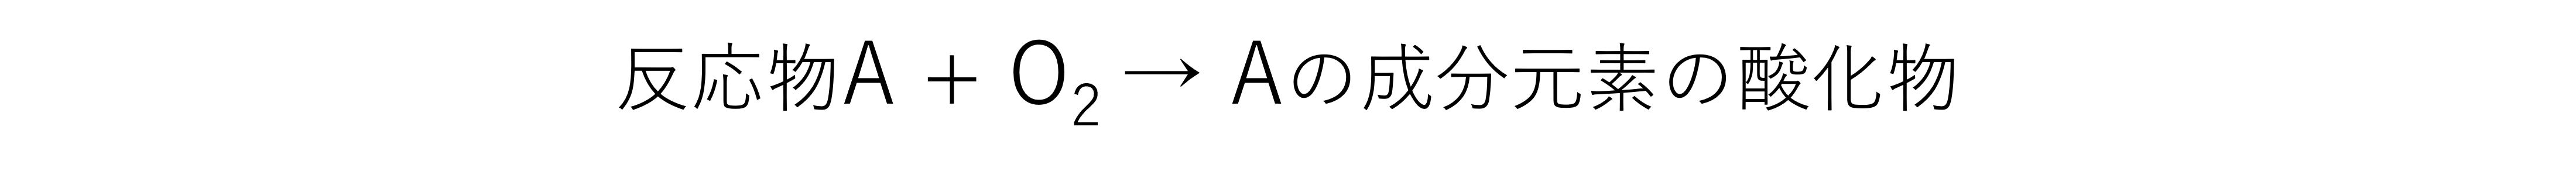
\includegraphics[width=1\linewidth]{asset/8.png}
  \end{figure}
\vspace*{-0.1cm}

\begin{enumerate}[1.]
  \item
  アルカリ金属(M)と酸素の反応\\
  \hspace*{10pt}{\large \ce{4 M + O2 -> 2 M2O}}
  \item
  アルカリ土類金属(M)と酸素の反応\\
  \hspace*{10pt}{\large \ce{2 M + O2 -> 2 MO}}
  \item
  アルミニウムと酸素の反応\\
  \hspace*{10pt}{\large \ce{4 Al + 3 O2 -> 2 Al2O3}}
  \item
  硫黄の燃焼反応\\
  \hspace*{10pt}{\large \ce{S + O2 ->[$\Delta$] SO2}}
  \item
  リンの燃焼反応\\
  \hspace*{10pt}{\large \ce{4 P + 5 O2 -> P4O10}}
  \item
  アルカンの燃焼反応\\
  \hspace*{10pt}{\large \ce{C_nH_{2n+2} + $\frac{{3 n + 1}}{2}$O2 ->[$\Delta$] n CO2 + ${(n + 1)}$ H2O}}
  \item
  二酸化硫黄と酸素の反応\\
  \hspace*{10pt}{\large \ce{2 SO2 + O2 ->[$\Delta$][\ce{V2O5}] 2 SO3}}
  \item
  硫化水素の燃焼反応\\
  \hspace*{10pt}{\large \ce{2 H2S + 3 O2 ->[$\Delta$] 2 SO2 + 2 H2O}}
  \item
  アンモニアを白金触媒を用いて,約900$\degree$ で空気酸化する\\
  \hspace*{10pt}{\large \ce{4 NH3 + 5 O2 ->[$\Delta$][\ce{Pt}] 4 NO + 6 H2O}}
  \item
  一酸化窒素と酸素を混合する\\
  \hspace*{10pt}{\large \ce{2 NO + O2 -> 2 NO2}}
  \item
  黄鉄鉱の燃焼反応\\
  \hspace*{10pt}{\large \ce{4 FeS2 + 11 O2 ->[$\Delta$] 2 Fe2O3 + 8 SO2}}
  \item
  硫化亜鉛の燃焼反応\\
  \hspace*{10pt}{\large \ce{2 ZnS + 3 O2 ->[$\Delta$] 2 ZnO + 2 SO2}}
\end{enumerate}

\vskip.5cm
\section*{自己酸化還元反応:}


\begin{enumerate}[1.]
  \item
  塩素を水に通じる\\
  \hspace*{10pt}{\large \ce{Cl2 + H2O <=> HCl + HClO}}\\
  \hspace*{10pt}補足:\\
  \hspace*{10pt}臭素も同様\ce{Br2 + H2O <=> HBr + HBrO}
  \item
  塩素を水酸化カルシウム水溶液に通じる\\
  \hspace*{10pt}{\large \ce{Cl2 + Ca(OH)2 -> CaCl(ClO)\cdot H2O}}
  \item
  塩素酸カリウム二酸化マンガン(IV)を加えて加熱する\\
  \hspace*{10pt}{\large \ce{2KClO3 ->[$\Delta$][\ce{MnO2}] 2 KCl + 3 O2}}
  \item
  過酸化水素水二酸化マンガン(IV)を加える\\
  \hspace*{10pt}{\large \ce{2 H2O2 ->[][\ce{MnO2}] 2 H2O + O2}}
  \item
  亜硝酸アンモニウム水溶液を加熱する\\
  \hspace*{10pt}{\large \ce{NH4NO2 ->[$\Delta$] 2 H2O + N2}}
  \item
  ハロゲン化銀に光を当てる\\
  \hspace*{10pt}{\large \ce{2AgX ->[\text{光}] 2 Ag + X2}}\\
  \hspace*{10pt}補足:\\
  \hspace*{10pt}光のエネルギーで黒色に変化する(感光性)
\end{enumerate}

\vskip.5cm
\section*{揮発性酸遊離反応:}
\vspace*{-0.5cm}
  \begin{figure}[H]\centering
    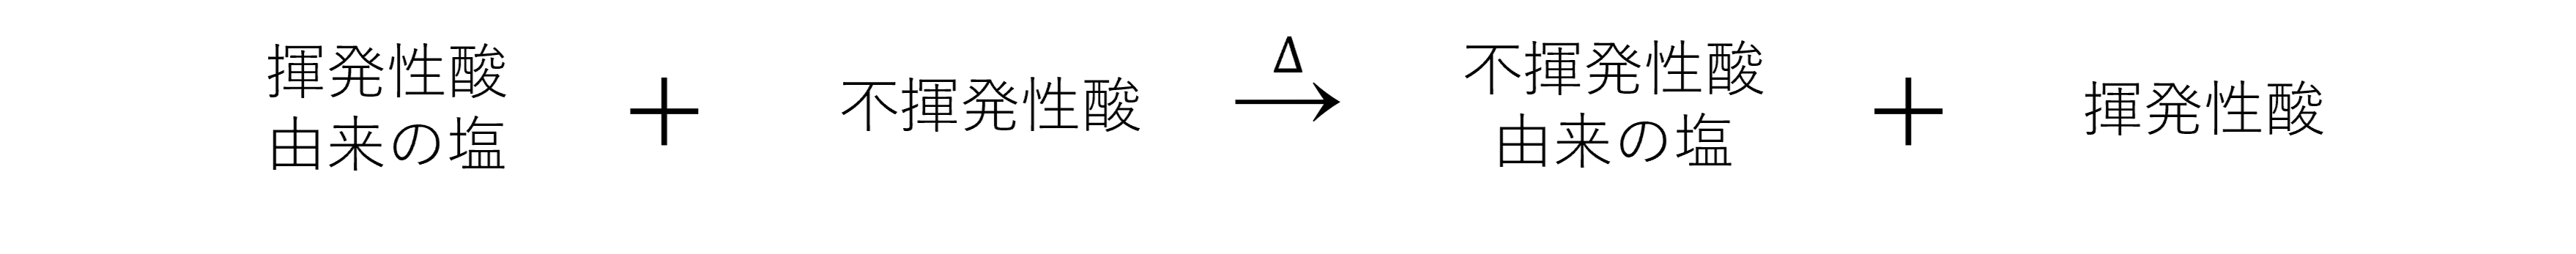
\includegraphics[width=1\linewidth]{asset/10.png}
  \end{figure}
\vspace*{-0.1cm}

\begin{enumerate}[1.]
  \item
  塩化ナトリウムの固体に濃硫酸を加えて加熱する\\
  \hspace*{10pt}{\large \ce{NaCl + H2SO4 ->[$\Delta$] NaHSO4 + HCl}}
  \item
  硝酸ナトリウムの固体に濃硫酸を加えて加熱する\\
  \hspace*{10pt}{\large \ce{NaNO3 + H2SO4 ->[$\Delta$] NaHSO4 + HNO3}}
  \item
  フッ化カルシウム(ホタル石)の固体に濃硫酸を加えて加熱する\\
  \hspace*{10pt}{\large \ce{CaF2 + H2SO4 ->[$\Delta$] CaSO4 + 2 HF}}
\end{enumerate}

\vskip.5cm
\section*{熱分解反応:}
\vspace*{-1cm}
  \begin{figure}[H]\centering
    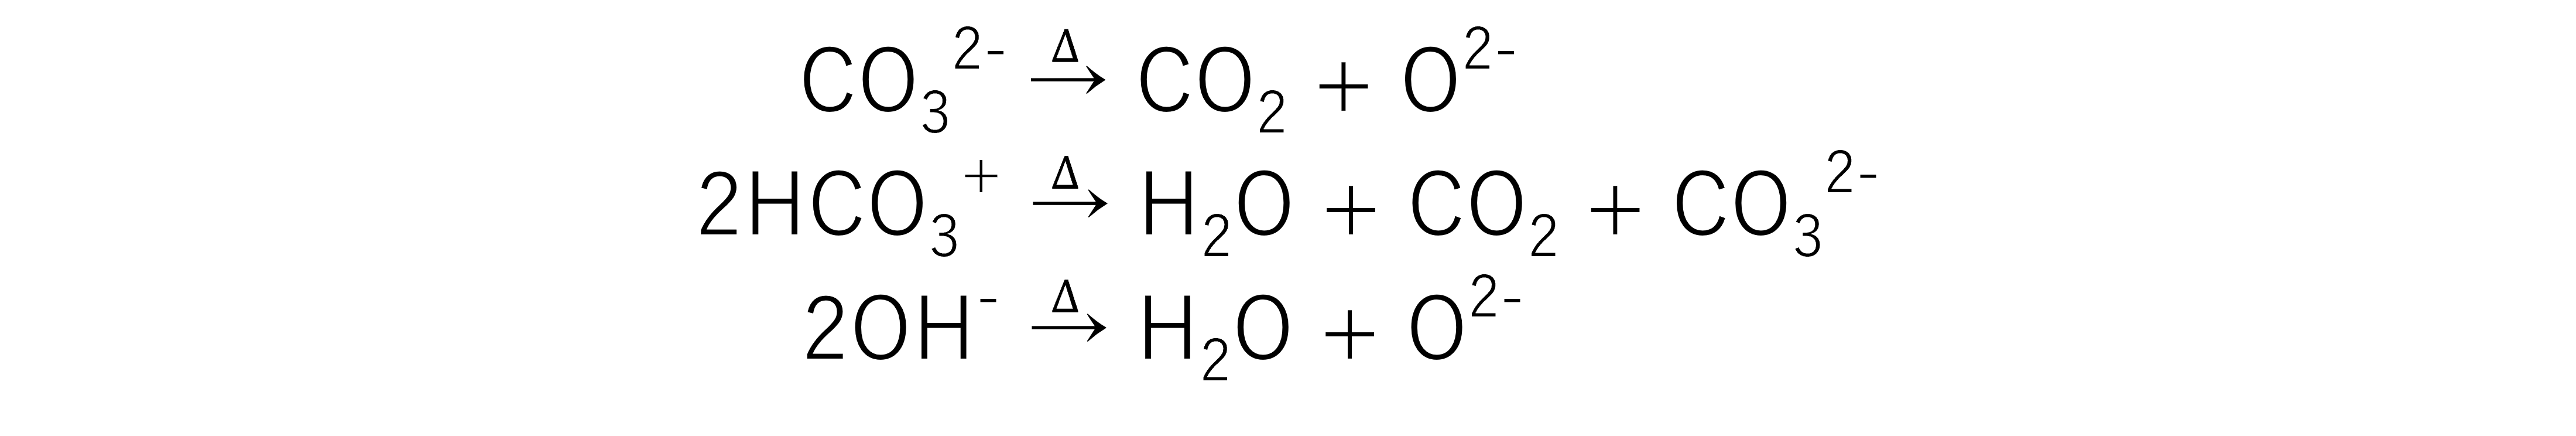
\includegraphics[width=1\linewidth]{asset/11.png}
  \end{figure}
\vspace*{-0.1cm}

\begin{enumerate}[1.]
  \item
  炭酸カルシウムを加熱する\\
  \hspace*{10pt}{\large \ce{CaCO3 ->[$\Delta$] CaO + CO2}}
  \item
  炭酸ナトリウムと二酸化ケイ素を混合して加熱する\\
  \hspace*{10pt}{\large \ce{Na2CO3 + SiO2 ->[$\Delta$] Na2SiO3 + CO2}}
  \item
  炭酸水素ナトリウム(重曹)を加熱する\\
  \hspace*{10pt}{\large \ce{2NaHCO3 ->[$\Delta$] Na2CO3 + H2O + CO2}}
  \item
  炭酸水素カルシウム水溶液を加熱する\\
  \hspace*{10pt}{\large \ce{Ca(HCO3)2 ->[$\Delta$] CaCO3 + H2O + CO2}}
  \item
  水酸化アルミニウムを加熱する\\
  \hspace*{10pt}{\large \ce{2 Al(OH)3 ->[$\Delta$] Al2O3 + 3H2O}}
  \item
  水酸化鉄(Ⅲ)を加熱する\\
  \hspace*{10pt}{\large \ce{2Fe(OH)3 ->[$\Delta$] Fe2O3 + 3 H2O}}
  \item
  水酸化銅(Ⅱ)を加熱する\\
  \hspace*{10pt}{\large \ce{Cu(OH)2 ->[$\Delta$] CuO + H2O}}
\end{enumerate}

\vskip.5cm
\section*{沈殿生成反応:}
\vspace*{-1cm}
  \begin{figure}[H]\centering
    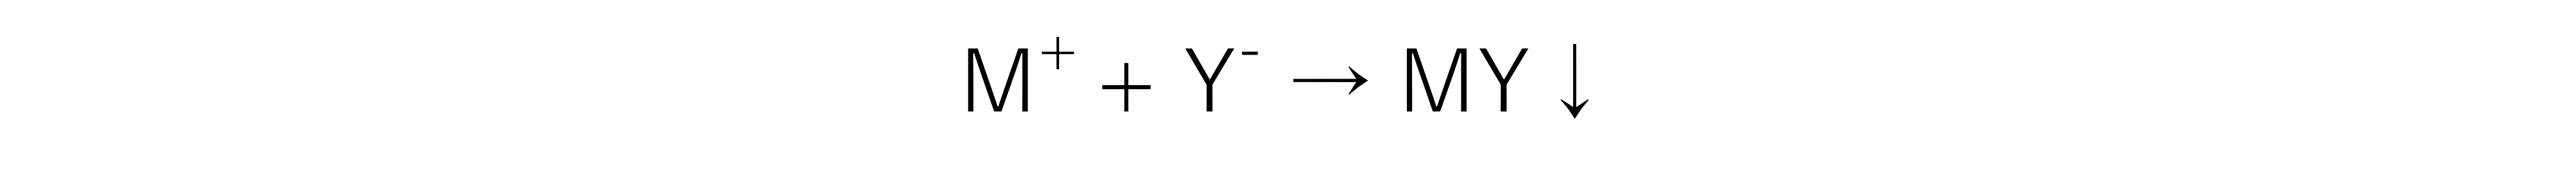
\includegraphics[width=1\linewidth]{asset/12.png}
  \end{figure}
\vspace*{-0.1cm}

\begin{enumerate}[1.]
  \item
  飽和食塩水にアンモニアと二酸化炭素を溶かす\\
  \hspace*{10pt}{\large \ce{NaCl + H2O + NH3 + CO2 -> NaHCO3 + NH4Cl}}
  \item
  金属陽イオン(\ce{Ag+},\ce{Al^{3+}},\ce{Cu^{2+}},\ce{Fe^{3+}})と水酸化物イオンとの反応\\
  \hspace*{10pt}{\large \ce{2 Ag+ + 2 OH- -> Ag2O + H2O}} \quad(\ce{Ag2O}:褐色) \\
  \hspace*{10pt}{\large \ce{Al^{3+} + 3 OH- -> Al(OH)3}} \quad(\ce{Al(OH)3}:白色) \\
  \hspace*{10pt}{\large \ce{Cu^{2+} + 2 OH^- -> Cu(OH)2}} \quad(\ce{Cu(OH)2}:青白色) \\
  \hspace*{10pt}{\large \ce{Fe^{3+} + 3 OH- -> Fe(OH)3}} \quad(\ce{Fe(OH)3}:赤褐色)
  \item
  金属陽イオン(\ce{Ag+},\ce{Cu^{2+}},\ce{Fe^{2+}},\ce{Zn^{2+}},\ce{Pb^{2+}})と硫化水素との反応\\
  \hspace*{10pt}{\large \ce{2 Ag+ + H2S -> Ag2S + 2 H+}} \quad(\ce{Ag2S}:黒色)\\
  \hspace*{10pt}{\large \ce{Cu^{2+} + H2S -> CuS + 2 H+}} \quad(\ce{CuS}:黒色)\\
  \hspace*{10pt}{\large \ce{Fe^{2+} + H2S -> FeS + 2 H+}} \quad(\ce{FeS}:黒色)\\
  \hspace*{10pt}{\large \ce{Zn^{2+} + H2S -> ZnS + 2 H+}} \quad(\ce{ZnS}:白色)\\
  \hspace*{10pt}{\large \ce{Pb^{2+} + H2S -> PbS + 2 H+}} \quad(\ce{PbS}:黒色)
  \item
  銀イオンと塩化物イオン,臭化物イオン,クロム酸イオンとの反応\\
  \hspace*{10pt}{\large \ce{Ag+ + Cl- -> AgCl}} \quad(\ce{AgCl}:白色) \\
  \hspace*{10pt}{\large \ce{Ag+ + Br- -> AgBr}} \quad(\ce{AgBr}:淡黄色)\\
  \hspace*{10pt}{\large \ce{2 Ag+ + CrO4^{2-} -> AgCrO4}} \quad(\ce{Ag2CrO4}:暗赤色)
  \item
  バリウムイオンと炭酸イオン,硫酸イオン,クロム酸イオンとの反応\\
  \hspace*{10pt}{\large \ce{Ba^{2+} + CO3^{2-} -> BaCO3}} \quad(\ce{BaCO3}:白色)\\
  \hspace*{10pt}{\large \ce{Ba^{2+} + SO4^{2-} -> BaSO4}} \quad(\ce{BaSO4}:白色)\\
  \hspace*{10pt}{\large \ce{Ba^{2+} + CrO4^{2-} -> BaCrO4}} \quad(\ce{BaCrO4}:黄色)
  \item
  鉛(Ⅱ)イオンと硫酸イオン,クロム酸イオン,塩化物イオンとの反応\\
  \hspace*{10pt}{\large \ce{Pb^{2+} + SO4^{2-} -> PbSO4}} \quad(\ce{PbSO4}:白色)\\
  \hspace*{10pt}{\large \ce{Pb^{2+} + CrO4^{2-} -> PbCrO4}} \quad(\ce{PbCrO4}:黄色)\\
  \hspace*{10pt}{\large \ce{Pb^{2+} + 2 Cl- -> PbCl2}} \quad(\ce{PbCl2}:白色沈殿,熱水に溶ける)
\end{enumerate}

  \begin{figure}[H]\centering
    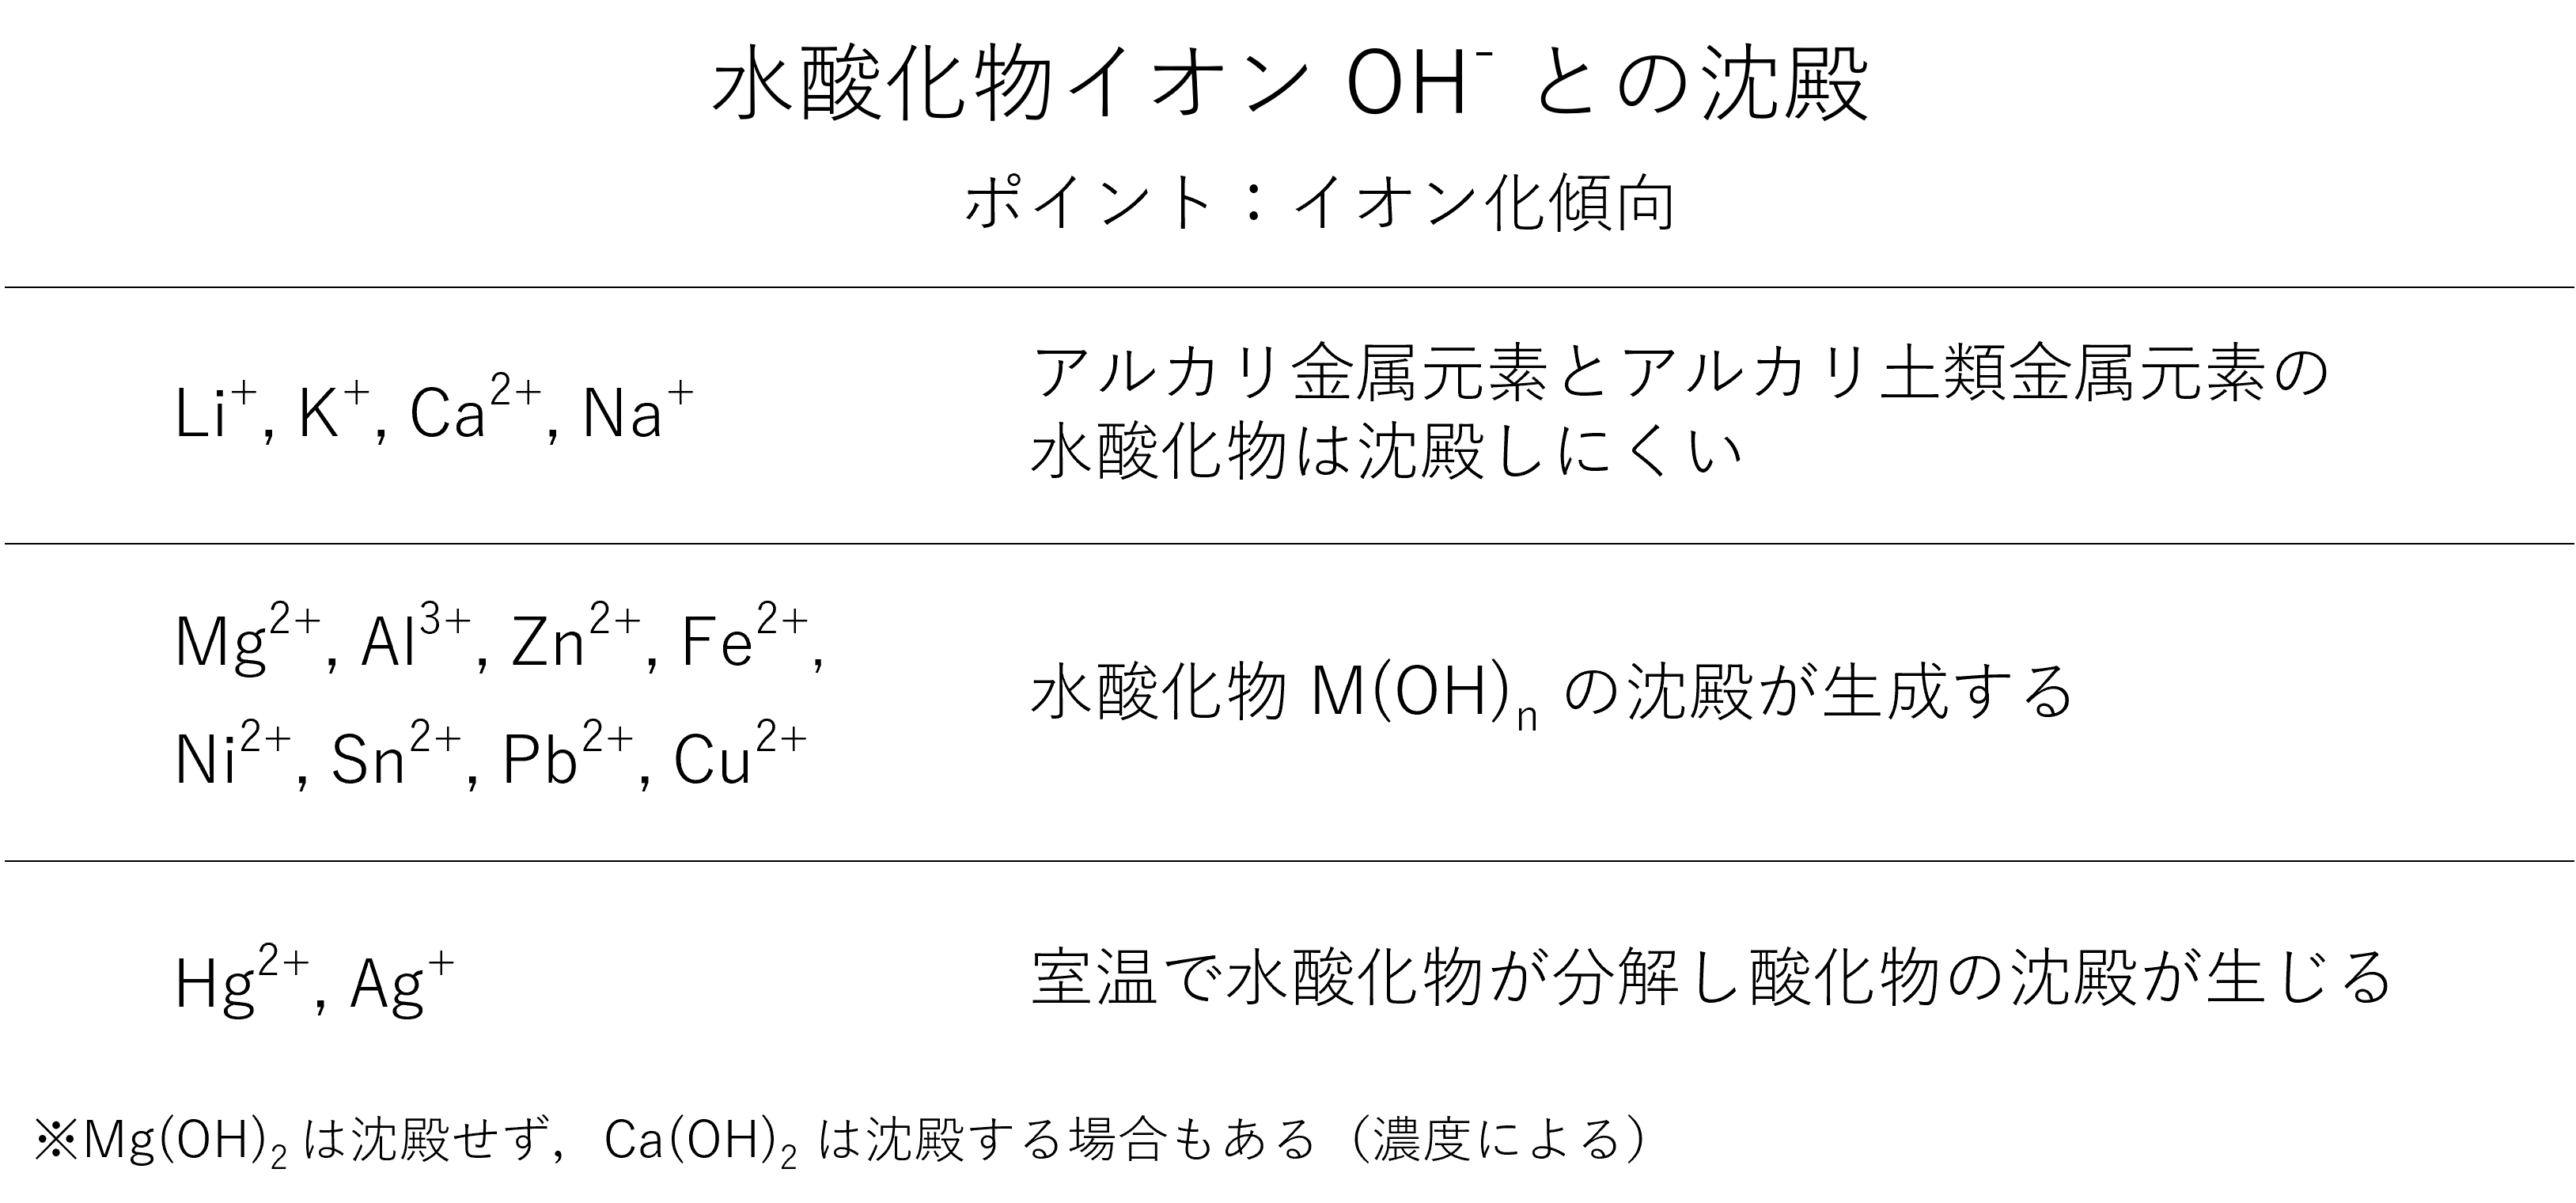
\includegraphics[width=1\linewidth]{asset/precipitation_table_OH.png}
  \end{figure}

  \begin{figure}[H]\centering
    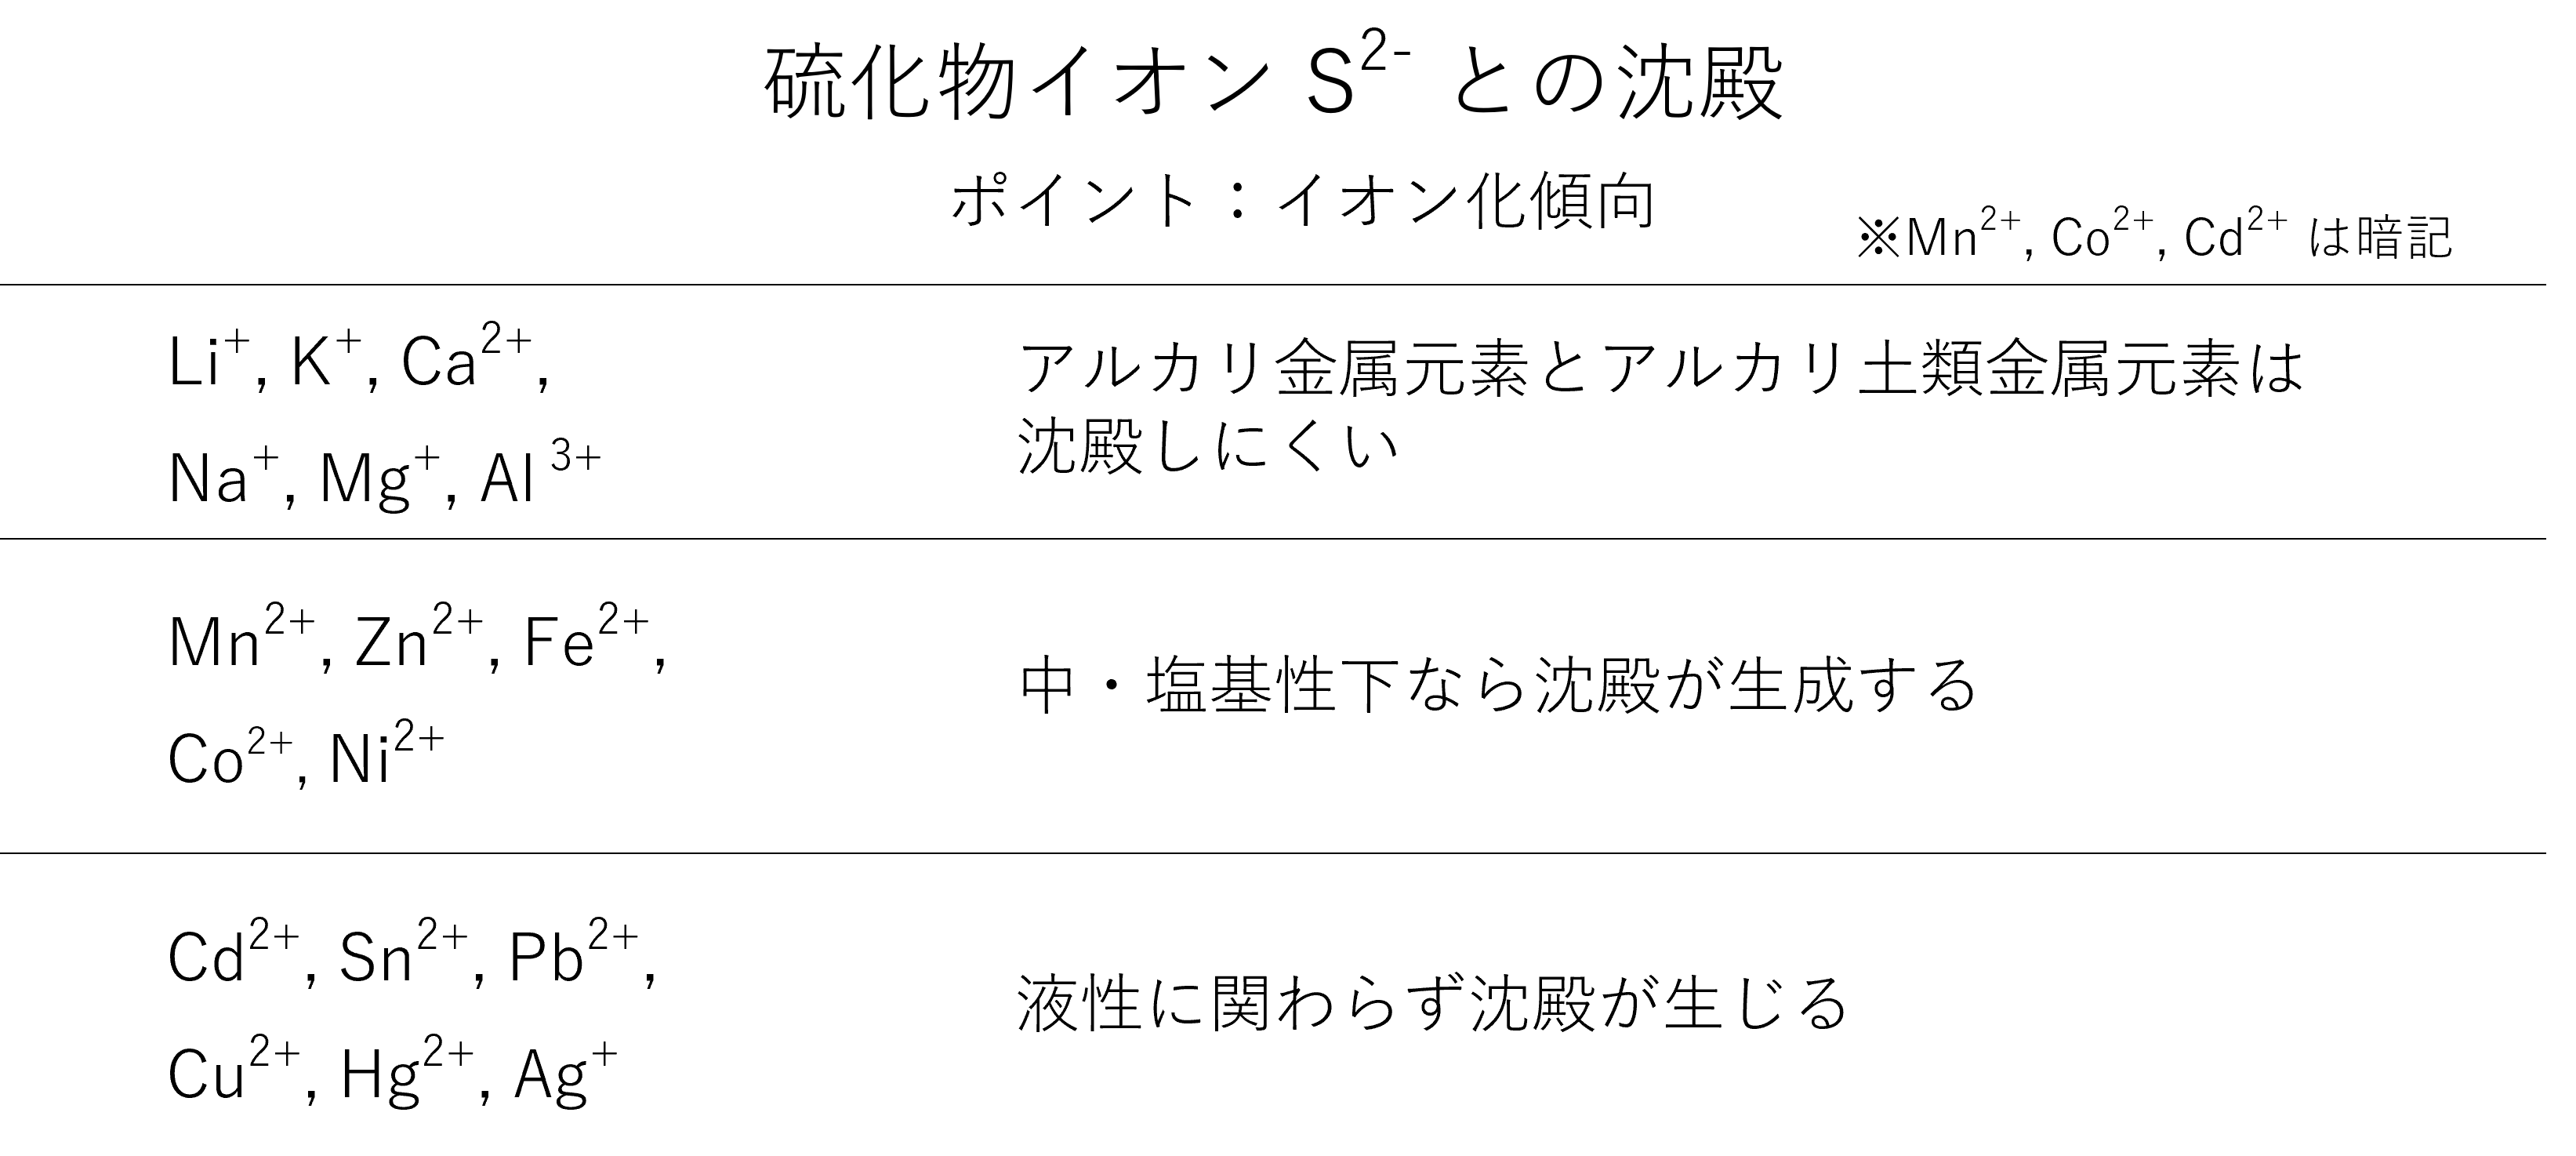
\includegraphics[width=1\linewidth]{asset/precipitation_table_S.png}
  \end{figure}



\vskip.5cm
\section*{錯イオン形成反応:}
\vspace*{-1cm}
  \begin{figure}[H]\centering
    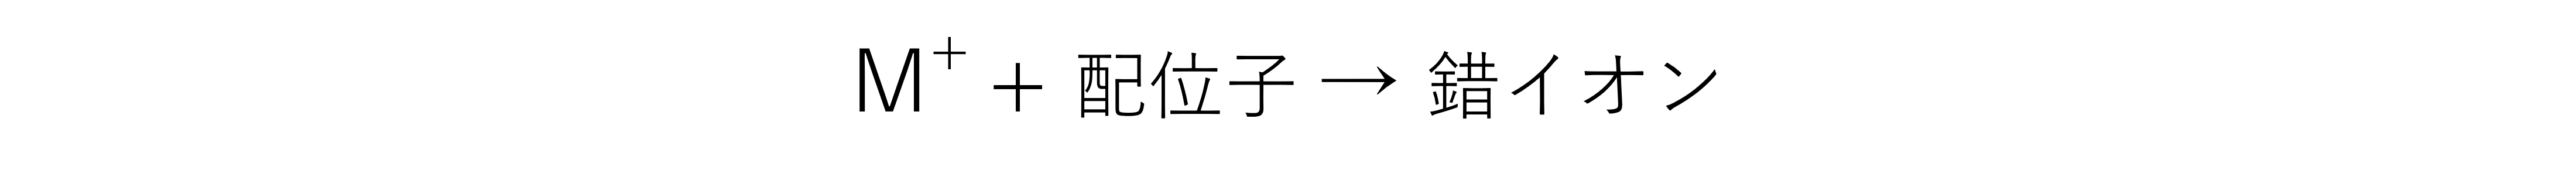
\includegraphics[width=1\linewidth]{asset/13.png}
  \end{figure}
\vspace*{-0.1cm}

\begin{enumerate}[1.]
  \item
  ガラスの主成分である二酸化ケイ素にフッ化水素酸を加える\\
  \hspace*{10pt}{\large \ce{SiO2 + 6HF -> H2SiF6 + 2 H2O}}\\
  \hspace*{10pt}補足: \\
  \hspace*{10pt}フッ化水素酸:フッ化水素の水溶液 \\
  \hspace*{10pt}\ce{H2SiF6}:ヘキサフルオロケイ酸 \\
  \hspace*{10pt}気体のフッ化水素では次の反応が起こる \\
  \hspace*{10pt}\ce{SiO2 + 4HF -> SiF4 + 2 H2O}
  \item
  亜鉛に水酸化ナトリウム水溶液を加える\\
  \hspace*{10pt}{\large \ce{Zn + 2 NaOH + 2 H2O -> Na2[Zn(OH)4] + H2}}
  \item
  アルミニウムに水酸化ナトリウム水溶液を加える\\
  \hspace*{10pt}{\large \ce{2 Al + 2 NaOH + 6 H2O -> 2 Na[Al(OH)4] + 3 H2}}
  \item
  酸化アルミニウムに水酸化ナトリウム水溶液を加える\\
  \hspace*{10pt}{\large \ce{Al2O3 + 3 NaOH + 3 H2O -> 2 Na[Al(OH)4]}}
  \item
  酸化亜鉛に水酸化ナトリウム水溶液を加える\\
  \hspace*{10pt}{\large \ce{ZnO + 2 NaOH + H2O -> Na2[Zn(OH)4]}}
  \item
  水酸化アルミニウムに水酸化ナトリウム水溶液を加える\\
  \hspace*{10pt}{\large \ce{Al(OH)3 + NaOH -> Na[Al(OH)4]}}
  \item
  水酸化亜鉛に水酸化ナトリウム水溶液を加える\\
  \hspace*{10pt}{\large \ce{Zn(OH)2 + 2 NaOH -> Na2[Zn(OH)4]}}
  \item
  過剰のアンモニア水と水酸化銅(Ⅱ),水酸化亜鉛,酸化銀,塩化銀との反応\\
  \hspace*{10pt}{\large \ce{Cu(OH)2 + 4 NH3 -> [Cu(NH3)4]^{2+} + 2 OH-}} \\
  \hspace*{10pt}{\large \ce{Zn(OH)2 + 4 NH3 -> [Zn(NH3)4]^{2+} + 2 OH-}} \\
  \hspace*{10pt}{\large \ce{Ag2O + H2O + 4 NH3 -> 2[Ag(NH3)2]+ + 2 OH-}} \\
  \hspace*{10pt}{\large \ce{AgCl + 2 NH3 -> [Ag(NH3)2]+ + Cl-}}
  \item
  塩化銀または臭化銀にチオ硫酸ナトリウム水溶液を加える\\
  \hspace*{10pt}{\large \ce{AgCl + 2 Na2S2O3 -> Na3[Ag(S2O3)2] + NaCl}} \\
  \hspace*{10pt}{\large \ce{AgBr + 2 Na2S2O3 -> Na3[Ag(S2O3)2] + NaBr}}
\end{enumerate}

\end{document}
